\section{Introduction}

When the data you want to model is high-dimensional, that is, the number of features \(p\)
exceed the number of observations \(n\), it is impossible to apply classical statistical
models such as standard linear regression since the design matrix \(\mat X\) is no longer
of full rank. A common remedy to this problem is to \emph{regularize} the model by adding a
term to the objective function that punishes models with large coefficients
(\(\vec\beta\)). If we let \(g(\vec\beta; \mat X, \vec y)\) be the original objective
function---which when minimized improves the model's fit to the data (\(\mat X, \vec
y\))---then we are interested in minimizing the following objective:
\begin{equation}
  \label{eq:general-objective}
  f(\beta_0, \vec\beta; \mat X, \vec y) = g(\beta_0, \vec\beta; \mat X, \vec y) + h(\vec\beta),
\end{equation}
which is composed of \(g\) and a penalty term \(h(\vec\beta)\). In
contrast to former, this penalty depends only on \(\vec{\beta}\).\footnote{Note that
  we do not penalize the intercept \(\beta_0\).}

Some of the most common penalties are the \(\ell_1\) norm and squared \(\ell_2\) norm
penalties, that is \(h(\vec\beta) = \lVert \vec\beta \rVert_1\) or \(h(\vec\beta) = \lVert
\vec\beta \rVert_2^2/2\)\footnote{Division by two in this case is used only for
  convenience.}, which, if \(g\) is the standard ordinary least-squares objective, represent
the lasso~\citep{tibshirani1996,santosa1986,donoho1994} and ridge (Tikhonov) regression
respectively. Other common penalities include the sorted \(\ell_1\)-norm used in Sorted
L-One Penalized Estimation (SLOPE)~\citep{bogdan2013,bogdan2015}, the minimax-concave
penalty (MCP)~\citep{zhang2010}, hinge loss (used in support vector
machines~\citep{cortes1995}) and smoothly-clipped absolute
deviation~(SCAD)~\citep{fan2001}. Many penalities---indeed all of the mentioned
ones---shrink coefficients in proportion to their sizes.

The issue with this type of shrinkage is that it is sensitive to the scales of the features
in \(\mat X\). To remedy this, it is common to \emph{normalize} the features before fitting
the model by shifting and dividing each column by respective centering and scaling factors.
For some problems such factors arise naturally from contextual knowledge about the problem
at hand, but in most cases they must be estimated from data. A popular stategy is to
translate by the mean of each feature and scale by the standard deviation, which is called
\emph{standardization}. Most types of normalization are based only on the marginal
distributions of the features, but there are exceptions such as the adaptive
lasso~\citep{zou2006}. Another reason for normalizing the features is to improve properties
of optimization algorithms used to fit the model, but we will not consider this topic here.

The choice of normalization may have consequences for the estimated model. As a first
example of this, consider \Cref{fig:realdata-paths}, which displays the lasso paths for
four real data sets and two different types of normalization. For most of the datasets, the
models differ significantly depending on type of normalization, yielding differences in
terms of feature selection as well as signs and magnitudes of the corresponding
coefficients.

\begin{figure}[bpt]
  \centering
  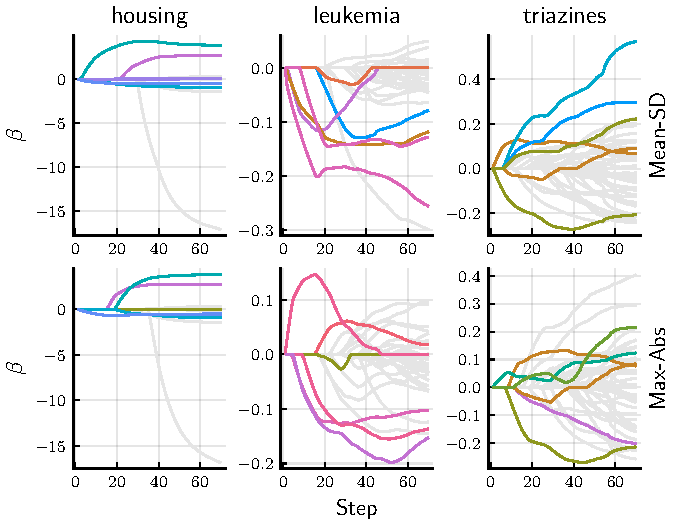
\includegraphics[]{plots/realdata_paths.pdf}
  \caption{%
    Lasso paths for real datasets using two types of normalization:
    standardization and maximum absolute value scaling (max--abs). We have fit
    the lasso path to four different datasets:
    \data{housing}~\citep{harrison1978}, \data{leukemia}~\citep{golub1999},
    \data{triazines}~\citep{king}, and \data{w1a}~\citep{platt1998}. For each
    dataset, we have colored the coefficients if they were among the first five
    to become non-zero under either of the two normalization schemes. We see
    that the paths differ with regards to the size as well as the signs of the
    coefficients, and that, in addition, the features to become active first
    differ between the normalization types.
  }
  \label{fig:realdata-paths}
\end{figure}

In spite of this strong relationship between normalization and regularization, there has so
far been no research on the topic. Instead, the choice of motivation is typically motivated
by being standard. Other times recommendations are based on computational aspects such as
optimization performance and data storage. At the time of writing, for instance, the
popular machine learning library \texttt{scikit-learn}~\citep{scikit-learndevelopers2024}
recommends max--abs scaling in the particular case of sparse data. Yet, as we have already
seen (\Cref{fig:realdata-paths}), this may have dramatic effects for the results.

Standardization is a natural choice when the features are normally distributed. For other
types of data, however, no such obvious choice exists. There is for instance no consensus
on how to normalize binary features (where the data take either of two values). Anecdotal
suggestions include not normalizing at all or to normalize as you would if it were
continuous data, but the implications of either of these suggestions (or in deed any other)
have yet to be researched.

In this paper, we will start to fill in this knowledge gap in the field of normalization
and regularization by focusing on normalization in the context of binary data. We will
focus on three models that each correspond to a particular case of
\Cref{eq:general-objective}: the lasso, ridge, and elastic net~\citep{zou2005}. The latter
of these, the elastic net, is a generalization of the previous two, and is the optimization
problem of minimizing the following objective function:
\begin{equation*}
  \underbrace{\frac{1}{2} \lVert \vec y - \beta_0 - \tilde{\mat{X}}\vec{\beta} \rVert^2_2}_{g(\beta_0, \vec{\beta}; \mat{X}, \vec{y})}  + \underbrace{\lambda_1 \lVert \vec\beta \rVert_1 + \frac{\lambda_2}{2}\lVert \vec \beta \rVert_2^2}_{h(\vec{\beta})}.
\end{equation*}
%
Setting \(\lambda_1 = 0\), we obtain the ridge regression objective, whilst setting
\(\lambda_2 = 0\), we get the lasso. All of these methods have become staples in the field
of statistics and machine learning and are accompanied by a large body of theoretical work
and applications for real data.

We pay particular attention to the case when these binary features are imbalanced, that is,
have relatively many ones or zeroes. In this case, we demonstrate that the choice of
normalization directly influences the estimated regression coefficients and that this
effect is different for the lasso and ridge regression. In the case of he lasso, we show
that this bias can be mitigated by scaling with variance rather than standard deviation,
but that this that this comes at the cost of increased variance. For ridge regression, we
instead need to scale by standard deviation. In the case of the elastic net, however, we
show that there is no simple normalization method that can mitigate this bias but that it
is possible to circumvent it by instead weighting the penalty terms in the elastic net.

We also study the case of mixed data and show that the choice of normalization has implicit
consequences for the relative weighting of binary and normal features, even in the case
when the binary features are balanced. If we believe, for instance, that a unit change in
the binary variable should equal a certain change in the normal variable (say, two standard
deviations), then scaling must be modified to take this into account.

% TODO: complete this paragraph
Finally, we look at a simple case of interactions between normal and binary features, and
demonstrate what?

